\documentclass[thmcnt=section, 12pt, color=cyan]{my-elegantbook}

% index page
\usepackage{imakeidx}
\makeindex[columns=2, intoc, options=-s index_style.ist]

% title and author
\title{Graph Theory}
\author{Isaac FEI}

% reference file
\addbibresource{Graph Theory.bib} 

% image of the book cover
\cover{cover2}

\begin{document}

% Print title and cover page
\maketitle

%--------
% preface
%--------

\frontmatter
\section*{Preface}

When writing this book, I mainly refer to \parencite{bondyGraphTheoryApplications1976}, which covers both theoretical results and crucial applications in graph theory. 

%------------------------------

% Print table of contents
\tableofcontents
\mainmatter

%-------------------------------
% main document starts from here
%-------------------------------

%==============================

\chapter{Basic Concepts of Graphs}

%------------------------------

\section{Isomorphism}

Two graphs $G$ and $H$ are identical, written as $G = H$, if all their components are the same, that is, $V(G) = V(H)$, $E(G) = E(H)$ and $\psi_G = \psi_H$. Identical graphs of course share the same properties. However, a graph $H$ does not necessarily have to be exactly $G$ to preserve all its properties. The labels of the vertices and edges are immaterial.

\begin{definition}
    Two graphs $G$ and $H$ are said to be isomorphic, written as $G \cong H$, if there exist bijections $\theta: V(G) \to V(H)$ and $\phi: E(G) \to E(H)$ such that 
    \begin{align}
        \psi_G(e) = u v
        \implies \psi_H(\phi(e)) = \theta(u) \theta(v)
        \label{eq:1}
    \end{align}
    The ordered pair $(\theta, \phi)$ is called an \textbf{isomorphism}\index{isomorphism} between $G$ and $H$.
\end{definition}

\parencite{bondyGraphTheoryApplications1976} includes the reverse direction of \eqref{eq:1} in the definition, that is, 
\begin{align*}
    \psi_G(e) = u v
    \iff \psi_H(\phi(e)) = \theta(u) \theta(v)
\end{align*}
But the reverse direction is redundant. To see this, we suppose that $\psi_H(\phi(e)) = \theta(u) \theta(v)$ and $\psi_G(e) = xy$. By \eqref{eq:1}, we have $\psi_H(e) = \theta(x) \theta(y)$. It then follows that $\theta(u) \theta(v) = \theta(x) \theta(y)$. We have either $\theta(u) = \theta(x)$, $\theta(v) = \theta(y)$, or $\theta(u) \theta(y)$, $\theta(v) = \theta(x)$. Because $\theta$ is a bijection, either $u=x$, $v=y$, or $u=y$, $v=x$. Either way, we have $uv = xy$. Therefore, $\psi_G(e) = x y = u v$, which proves the reverse direction $\Leftarrow$.

For simple graphs, there is no need to find a bijection between edges once the bijection $\theta$ between vertices is established.

\begin{proposition} \label{pro:1}
    Let $G$ and $H$ be simple graphs. Then $G \cong H$ if and only if there exists a bijection $\theta: V(G) \to V(H)$ such that 
    \begin{align}
        u v \in E(G)
        \implies \theta(u) \theta(v) \in E(H)
        \label{eq:2}
    \end{align}
\end{proposition}

\begin{proof}
    (Necessity) Suppose that there exist $\theta$ and $\phi$ satisfying \eqref{eq:1}. If $e = u v \in E(G)$, then by \eqref{eq:1}, $\psi_H(\phi(e)) = \theta(u) \theta(v)$, which implies $\theta(u) \theta(v) \in E(H)$.

    (Sufficiency) Define $\phi: E(G) \to E(H)$ by 
    \begin{align*}
        \phi(u v) = \theta(u) \theta(v)
    \end{align*}
    We need to show $\phi$ is bijective. Suppose $\phi(u v) = \phi(x y)$. We have $\theta(u) \theta(v) = \theta(x) \theta(y)$. Applying a similar argument we used in the previous comments, we will finally obtain $u v = x y$, which means $\phi$ is injective. On the other hand, for any edge $f \in H$. Write $f = ij$ (i.e., $\psi_H(f) = ij$). Then because $\theta$ is bijective, there exist $u, v \in V(G)$ such that $\theta(u) = i$ and $\theta(v) = j$. Hence, $\phi(u v) = ij$, which implies $\phi$ is surjective.

    If $\psi(e) = uv$, i.e., $e = uv \in E(G)$, then we have $\theta(u) \theta(v) \in E(H)$ by \eqref{eq:2}. Equivalently, $\psi_H(\phi(e)) = \theta(u) \theta(v)$.
\end{proof}

%------------------------------

A \textbf{complete bipartite graph}\index{complete bipartite graph} is a \textit{simple} bipartite graph with bipartition $(X, Y)$ in which each vertex in $X$ is incident with each vertex in $Y$. That is, if $x \in X$ and $y \in Y$, then $xy \in E$. If $\abs{X} = m$ and $\abs{Y} = n$, we often use the symbol $K_{m,n}$ to denote this complete bipartite graph. (See Figure~\ref{fig:2}.) Note that this implicitly implies that the complete bipartite graph is unique in some way since we can represent it with a common symbol. Indeed, it is unique up to isomorphism, as we will show in the next proposition.

\begin{figure}[ht]
    \centering
    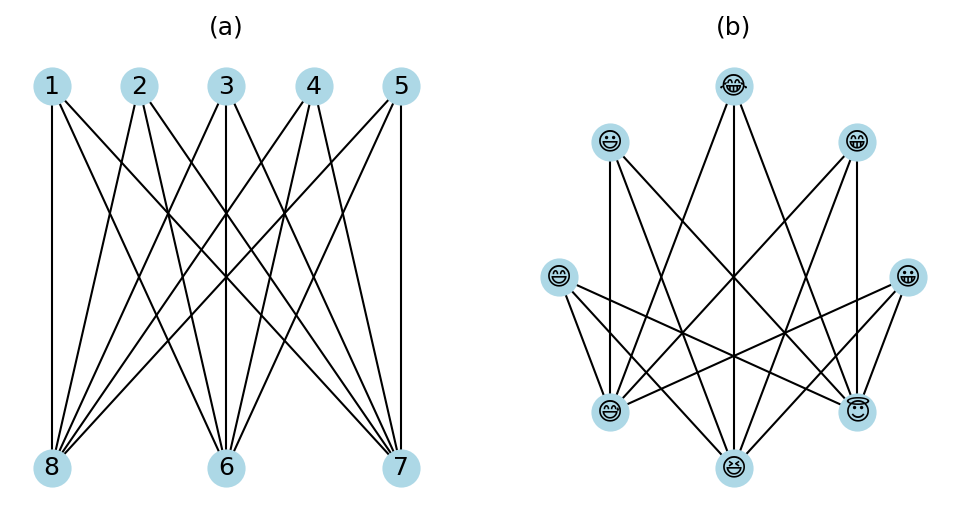
\includegraphics[scale=0.7]{figures/g-002.png}
    \caption{Both (a) and (b) are $K_{5,3}$.}
    \label{fig:2}
\end{figure}

\begin{proposition}
    Let $G[X, Y]$ and $H[U, V]$ be two complete bipartite graphs with $\abs{X} = \abs{U}$ and $\abs{Y} = \abs{V}$. Then $G \cong H$. In other words, a complete bipartite graph is unique up to isomorphism if the sizes of its two vertex sets in bipartition are determined.
\end{proposition}

\begin{proof}
    Since $\abs{X} = \abs{U}$ and $\abs{Y} = \abs{V}$, we can find a bijection $\theta: V(G) \to V(H)$ in such a way that $\theta$ maps each point in $X$ onto $U$, and each point in $Y$ onto $V$. Then for an edge $xy \in E(G)$, we have $\theta(x)\theta(y) \in E(H)$ since there has to be an edge connecting $\theta(x) \in U$ and $\theta(y) \in V$ by the definition of complete bipartite graphs. This proves $G \cong H$ by Proposition~\ref{pro:1}.
\end{proof}


%------------------------------

\section{Vertex Degrees}

%------------------------------





%------------------------------

\section{Paths and Connection}

%------------------------------

A \textbf{walk}\index{walk in a graph} in a graph is a sequence of edges $e_1 \cdots e_k$ joining a \textit{nonempty} sequence of vertices $v_0 v_1 \cdots v_k$, which is denoted by 
\begin{align}
    v_0 e_1 v_1 \cdots e_k v_k 
    \label{eq:3}
\end{align}
with each edge written after one of its end and followed by its other end. Note that though the sequence of vertices in a walk is required to be nonempty, the sequence of edges may be empty. And in that case, the walk contains only one vertex, say $v_0$, and it is called the \textbf{trivial walk}\index{trivial walk}.
\begin{note}
    The term \textbf{sequence} in mathematics often means an infinite sequence, which is essentially a function defined on $\N^\ast$. However, in graph theory, we usually refer to sequence as a \textbf{finite} list of ordered elements.
\end{note}

We call a walk $W$ from $v_0$ to $v_k$ a $(v_0, v_k)$-walk. The vertices $v_0$ and $v_k$ are referred to as the \textbf{origin}\index{origin of a walk} and the \textbf{terminus}\index{terminus of a walk} of that walk, respectively. 

It should be emphasized that neither the edges nor the vertices in a walk are necessarily distinct. However, if all edges of walk $W$ are distinct, we call $W$ a \textbf{trail}\index{trail in a graph}. And if all vertices in $W$ are distinct, it is then called a \textbf{path}\index{path in a graph}. Of course, all edges in a path are also distinct since the vertices are.

Two vertices are said to be \textbf{connected}\index{connected and disconnected vertices} if there exists a path joining them. Otherwise, they are \textbf{disconnected}. 

The length of a path $P$, written as $\abs{P}$, is defined as the number of edges along it. Note that the length of a trivial path is zero since there are no edges.

If $G$ is a simple graph, then we may write a walk simply as a sequence of vertices since there is one and only one edge joining each pair of consecutive vertices in the walk. For example, we write the $(v_0, v_k)$-walk in \eqref{eq:3} as 
\begin{align*}
    v_0 v_1 \cdots v_k
\end{align*}
with edges dropped.

%------------------------------

\begin{proposition} \label{pro:1}
    If there is a $(u, v)$-walk in $G$, then there is also a $(u, v)$-path in $G$.
\end{proposition}

This can be proved easily using the following algorithm (Algorithm~\ref{alg:1}).

\begin{algorithm}[ht]
    \KwIn{A walk $W = v_0 e_1 v_1 \cdots e_k v_k$}
    \KwOut{A path $P$}
    initialize $P$ as a sequence containing just one vertex $v_0$ \;
    \For{$i = 1, \ldots, k$}{
        \eIf{$v_i$ is not in $P$}{
            append $e_i$ and $v_i$ to $P$ \;
        }{
            remove all the vertices and edges after the vertex $v_i$ from $P$ \;
        }
    }
    \caption{Extracting a Path From a Walk}
    \label{alg:1}
\end{algorithm}

%------------------------------

\begin{proposition}
    The number $(v_i, v_j)$-walks of length $k$ in $G$ is the $(i,j)$-th entry of the $k$-th power of the adjacency matrix $A$, i.e., $A^k$.
\end{proposition}

\begin{proof}
    % TODO
\end{proof}

%------------------------------

\section{Cycles}

%------------------------------

One simple yet useful observation of a particular longest path 
in a graph is that all the neighbors of the terminus must 
occur along the path. To be specific, 
if $P = v_0 e_1 v_1 \cdots e_k v_k$ is one of the longest paths in $G$ 
then $P$ must contain all vertices in $N(v_k)$. 
To prove this, we assume $P$ does not contain $v_{k+1} \in N(v_k)$. 
(Suppose $\psi(e_{k+1}) = v_k v_{k+1}$.) 
Then the path $P + e_{k+1}v_{k+1}$ is clearly longer than $P$, 
which leads to a contradiction. 
Figure~\ref{fig:1} depicts such an example. 
Note that if $8$ were a neighbor of $7$, 
then path $12345678$ would be longer.

\begin{figure}[ht]
    \centering
    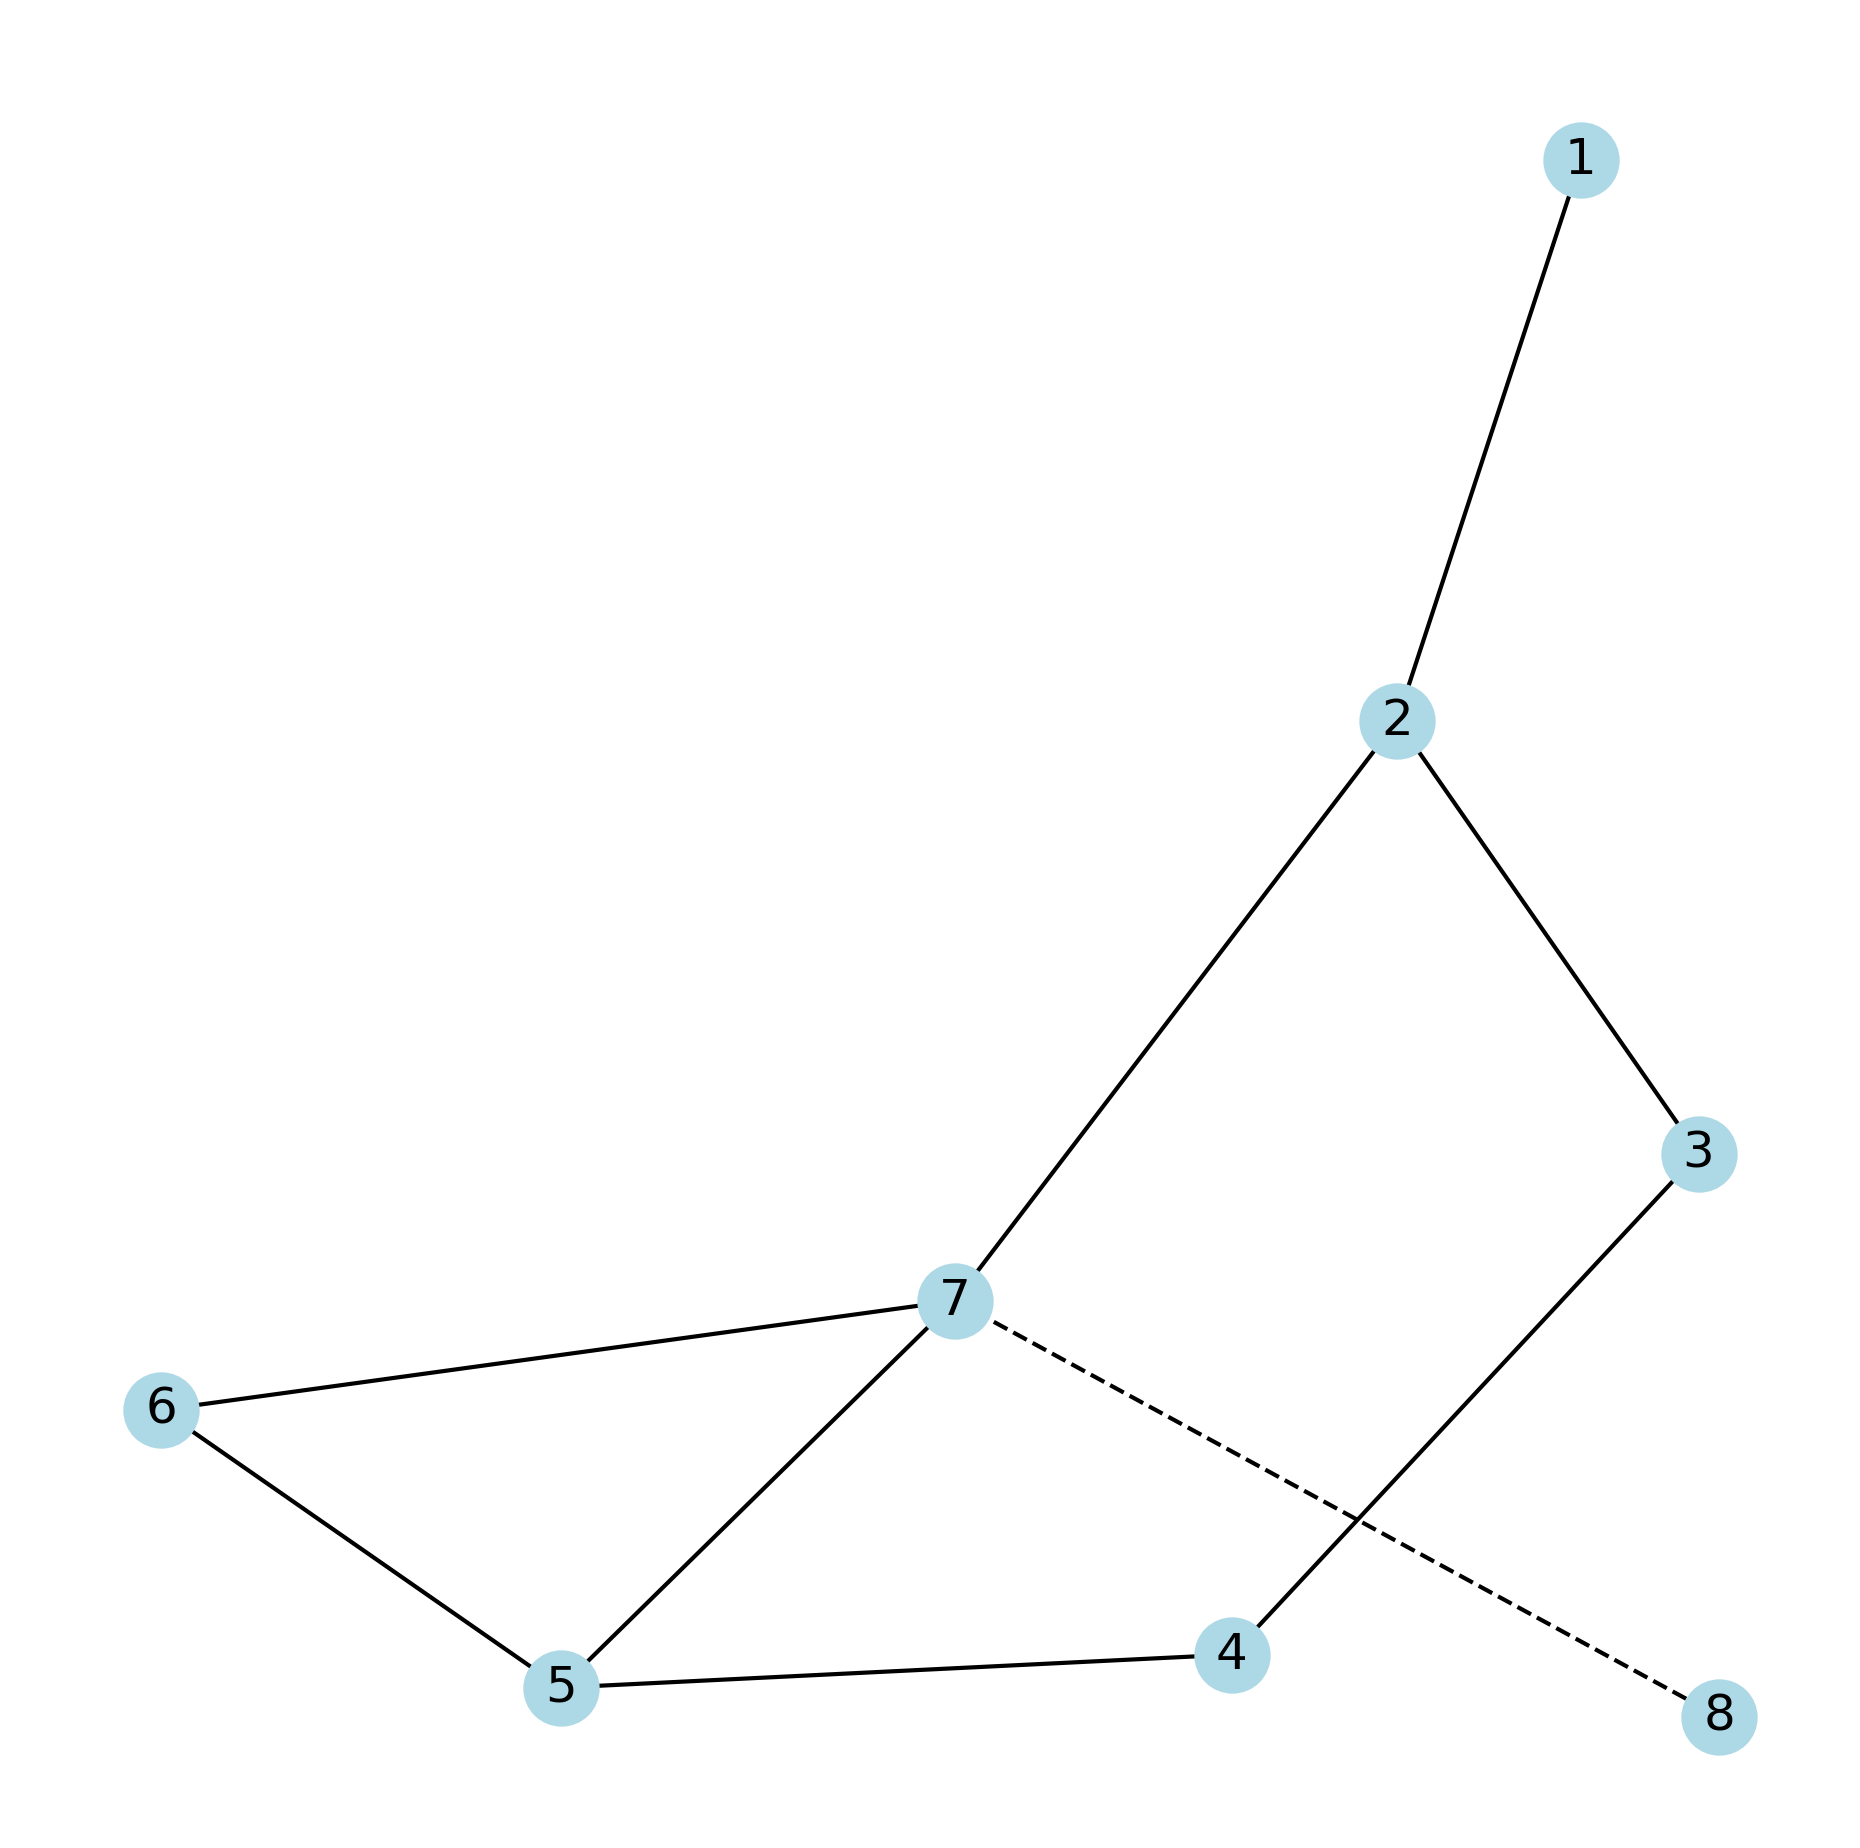
\includegraphics[scale=0.7]{figures/g-001.png}
    \caption{Path $1234567$ is one of the longest paths.}
    \label{fig:1}
\end{figure}

%------------------------------

\begin{proposition} \label{pro:5}
    If $G$ is a simple graph with $\delta(G) \geq 2$, 
	then there exists a cycle of length 
	at least $\delta(G)+1$.
\end{proposition}

\begin{proof}
	Let $P = u \cdots v$ 
	be a longest path in $G$.
	As noted before, all the neighbors of 
	the terminus $ v $,
	denoted by $v_1, \ldots, v_{\delta(G)}$
	arranged by their original order in $P$,
	must occur along the path $P$.
	Note that the $(v_1, v)$-section,
	denoted by $Q$,
	is of length $\delta(G)$.
	Notice also that $Q v_1$ is a cycle 
	since $v_1$ is incident with $v$.
	And it is of length $\delta(G) + 1$.
	This completes the proof.
\end{proof}

In fact, we have an algorithm to find a cycle without knowing the longest path in $G$.

\begin{algorithm}[ht]
    \KwIn{$G$ with $\delta(G) \geq 2$}
    \KwOut{A cycle $C$}
    \If{$G$ has a loop $e$ from $v$ to $v$}{
        $C \gets v e v$ \;
        \Return{$C$} \;
    }
    pick a vertex $v_0$ \; 
    $P \gets v_0$ \;
    pick $v \in N(v_0)$ and let $e$ be the corresponding edge, i.e., $\psi(e) = v_0 v$ \;
    \While{$v \notin P$}{
        $P \gets P e v$ \;
        pick $u \in N(v)$ such that
        there exists an edge $f$ satisfying $\psi(f) = v u$ and $f \neq e$ \;
        $v \gets u$ \; 
        $e \gets f$ \;
    }
    remove from $P$ all vertices and edges before $v$ \;
    $C \gets P e v$ \;
    \caption{Finding a Cycle in $G$ With $\delta(G) \geq 2$}
    \label{alg:2}
\end{algorithm}

\begin{proof}
We need to show that Algorithm~\ref{alg:2} works correctly. 
    
\noindent \textbf{Initialization:} Firstly, note that line 7 is possible 
since $v_0$ has no loops and $\deg(v_0) \geq 2$. 

We claim the loop invariants are
\begin{enumerate}
    \item $P$ has $j$ vertices assuming that 
		we are to execute the $j$-th iteration,
    \item $P$ has no duplicated vertices, i.e., $P$ is a path, and
    \item edge $e$ is incident with $v$.
\end{enumerate}

\noindent \textbf{Maintenance:} Suppose we are in the $j$-th iteration. 
After line 9, $P$ remains a path. Because $\deg(v) \geq 2$, 
there exists an edge $f$ other than $e$ that is incident with $v$. 
Hence, line 10 works correctly. 
After executing line 12, we find that the number of vertices in $P$ is increased by one, i.e., $j+1$, 
$P$ is still a path and $e$ is incident with $v$.

\noindent \textbf{Termination:} We can complete at most $n-1$ iterations 
since $P$ can hold at most as many vertices as there are in $G$. 
Upon termination, 
we find $v$ is in $P$ and $e$ is incident with $v$. 
By removing from $P$ all vertices and edges before $v$ 
and then append to it edge $e$ and vertex $v$, 
we will obtain a cycle from $v$ to itself. 
\end{proof}

%------------------------------

\begin{theorem} \label{thm:1}
    % TODO
\end{theorem}

%------------------------------

The \textbf{girth}\index{girth} of a graph is defined as 
the length of its shortest cycle.
We say the girth of $G$ is infinity if it contains no cycles.
Apparently, if $G$ has girth 1, then it contains a loop.
If it has girth 2, then there must be a parallel edge. 
But it has no loops.
And if the girth of $G$ is greater than or equal to 3,
then it must be a simple graph.

\begin{proposition}\label{pro:3}
	A $k$-regular graph with girth 4 has at least $2k$ vertices.
	Moreover, if it has exactly  $2k$ vertices, 
	then it must be $K_{k,k}$, i.e.,
	a complete bipartite graph with both sides of 
	the bipartition having the same size $k$.
	Conversely, $K_{k,k}$ is a $k$-regular graph with girth 4.
\end{proposition}

Figure~\ref{fig:3} depicts several $K_{k,k}$ graphs.

\begin{figure}[ht]
    \centering
    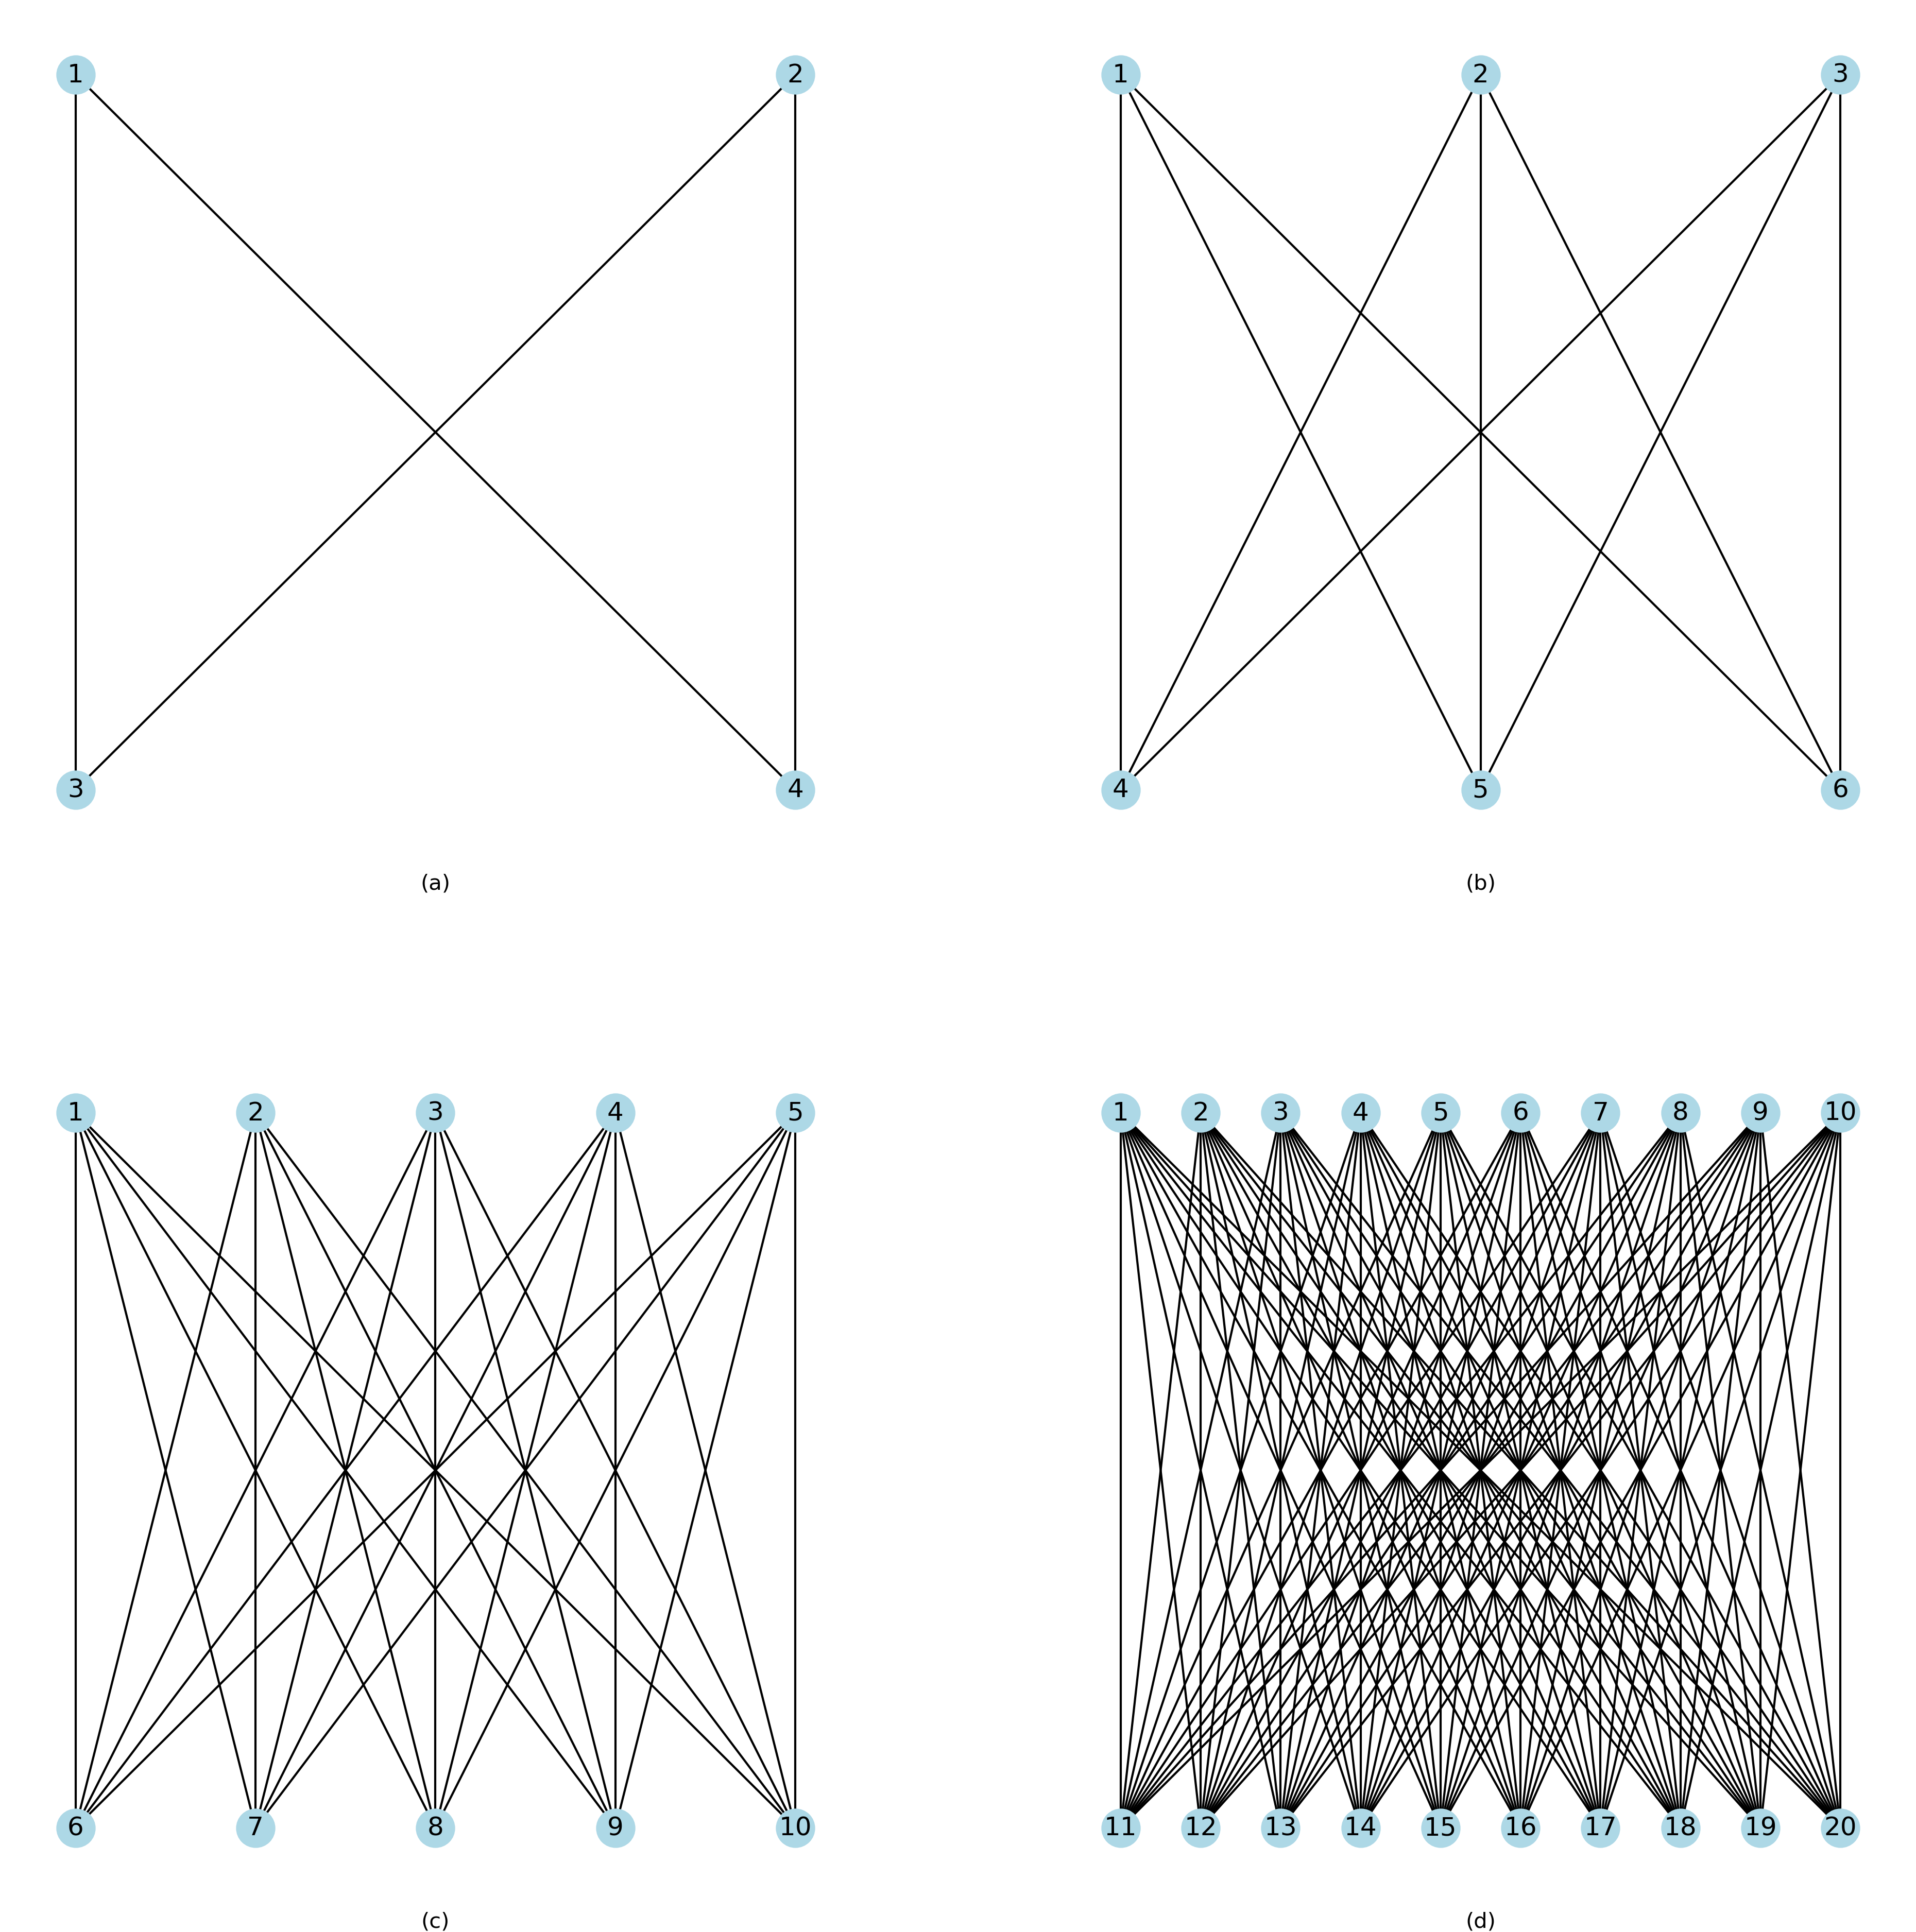
\includegraphics[scale=0.5]{figures/g-003.png}
	\caption{(a) $K_{2,2}$. (b) $K_{3,3}$. (c)  $K_{5,5}$. 
	(d)  $K_{10,10}$.}
    \label{fig:3}
\end{figure}

\begin{proof}
    Take a pair of incident vertices $u$ and $v$ in $G$.
	We have $N(u) \cap N(v) = \emptyset$. 
	Otherwise, a triangle would appear. 
	Because the degrees of $u$ and  $v$ are both $k$,
	equivalently, the sizes of their neighbors are $k$,
	$G$ must has at least $2k$ vertices 
	having these two disjoint sets $N(u)$ and $N(v)$.

	Suppose $\abs{V} = 2k$. 
	Pick a pair of incident vertices $u$ and $v$ as before.
	From the previous proof, we know
	$\abs{N(u)} = \abs{N(v)} = k$ and they are disjoint.
	Since  $G$ now only has  $2k$ vertices,
	$V$ is composed of
	these two neighbor sets, i.e., $V = N(u) \uplus N(v)$.
	Observe that each pair of vertices in  $N(u)$
	cannot be joined with each other for 
	there are no triangles.
	The same conclusion also holds for $N(v)$.
	Therefore, every vertex in 
	$N(u)$ is joined with every vertex in $N(v)$
	because the degree of every vertex is $k$.
	This shows that $G$ is  $K_{k,k}$.

	We also need to show $K_{k,k}$ is a $k$-regular graph with girth 4.
	Clearly, it is $k$-regular. 
	It contains no cycles with length 1 or 3 by Theorem~\ref{thm:1}.
	Of course, it does have any parallel edges, 
	hence no 2-cycles.
	And we can easily find a 4-cycle in it.
	For example, if we suppose 
	$X=\{x_1,\ldots,x_k\}$ and $Y=\{y_1,\ldots,y_k\}$ 
	form a bipartition of $K_{k,k}$, then 
	$x_1 y_1 x_2 y_2 x_1$ is a 4-cycle.
\end{proof}

%------------------------------

\section{Shortest Paths and Dijkstra's Algorithm}

With every edge $e$ in graph $G$, we can associate a real number $w(e)$, usually positive, which we shall call the \textbf{weight}\index{weight of an edge} of that edge. As we will see, to unify our notations for some special cases, it is convenient to define the weight of a nonexistent edge between two non-incident vertices as infinity $\infty$. 

We can now extend our former definition of the length of a path by 
\begin{align*}
    \abs{P} := \sum_{e \in P} w(e)
\end{align*}
Note that if all the edges are assigned to unit weights, then $\abs{P}$ is just the number of edges in it, which reduces to the former definition. Notice also that the length of a trivial path is also zero since the sum of nothing in the above equation, by convention, is zero.

Given a map, the cities can be regarded as vertices, and for each pair of adjacent cities, we can draw an edge in between them. In this example, it is reasonable to define the weight of edge $uv$ as the distance between cities $u$ and $v$. Then the problem of finding a shortest path from $u_0$ to $v$ arises quite naturally if we want to travel from city $u_0$ (where we live) to every other city $v$ at the minimum cost.

Formally, for all $u, v \in V$, the length of the shortest path from $u$ to $v$ is defined as 
\begin{align*}
    d(u,v) := 
    \begin{cases}
        \min \set{\abs{P}}{\text{$P$ is a $(u, v)$-path}} ,
        &\text{if $u$ and $v$ are connected} \\ 
        \infty,
        &\text{if $u$ and $v$ are disconnected}
    \end{cases}
\end{align*}
Given a proper subset $S$ of $V$ and a source $u_0 \in S$ in it, it is natural to define the distance from $u_0$ to the complement $S^\complement$ as the minimum distance from $u_0$ to every $v \in S^\complement$, that is,
\begin{align*}
    d(u_0, S^\complement) := \min_{v \in S^\complement} d(u_0, v)
\end{align*}
Of course, if $d(u_0, S^\complement) = \infty$, then there are no paths from $u_0$ to any vertex in $S^\complement$, in other words, $u_0$ is disconnected from $S^\complement$. Suppose $d(u_0, S^\complement)$ is a finite number, which means there exists a path $P = u_0 \cdots u v$ from $u_0$ to some vertex $v \in S^\complement$. The following are some simple observations about this path $P$:
\begin{enumerate}
    \item $P$ is a shortest $(u_0, v)$-path,
    \item $u \in S$ and the $(u_0, u)$-section, $u_0 \cdots u$, is a shortest $(u_0, u)$-path, and
    \item we have the equation
    \begin{align}
        d(u_0, S^\complement) = d(u_0, u) + w(uv)
        \label{eq:9}
    \end{align}
\end{enumerate}
Equation \eqref{eq:9} motivates us to state the following proposition, which is the central idea of Dijkstra's algorithm.

\begin{proposition} \label{pro:2}
    Let $G = (V, E)$ be a simple graph. Let $S \subseteq V$ be a subset of vertices and $u_0 \in S$ a point in it. We have 
    \begin{align}
        d(u_0, S^\complement)
        = \min_{u \in S, v \in S^\complement} \{
            d(u_0, u) + w(u v)
        \}
        \label{eq:5}
    \end{align}
\end{proposition}

\begin{proof}
    First, note that the set 
    \begin{align*}
        \set{d(u_0, u) + w(u v)}{u \in S, v \in S^\complement}
    \end{align*}
    is a finite set (possibly containing infinite numbers). Hence, it does have a minimum. 

    Assume there exist $u^\ast \in S$ and $v^\ast \in S^\complement$ such that 
    \begin{align}
        d(u_0, S^\complement)
        > d(u_0, u^\ast) + w(u^\ast v^\ast)
        \label{eq:4}
    \end{align}
    \begin{note}
        Note that \eqref{eq:4} implicitly implies that $u_0$ and $u^\ast$ are connected and $u^\ast$ and $v^\ast$ are connected since the right-hand side of \eqref{eq:4} is a finite number.
    \end{note}
    \noindent Then there exists a $(u_0, u^\ast)$-path $P$ such that $\abs{P} = d(u_0, u^\ast)$. Note that $P v^\ast$ forms a path since all vertices in $P$ are in $S$ while $v^\ast$ is in the complement $S^\ast$. But $P v^\ast$ is a path from $u_0$ to $S^\complement$ with length $d(u_0, u^\ast) + w(u^\ast v^\ast)$, which is less than $d(u_0, S^\complement)$ by assumption. Therefore, this leads to a contradiction. We have 
    \begin{align*}
        d(u_0, S^\complement)
        \leq d(u_0, u) + w(u v)
        \quad
        \forall u \in S \; 
        \forall v \in S^\complement
    \end{align*}
    And \eqref{eq:5} is proved.
\end{proof}

%------------------------------

\subsection{A First Attempt}

Starting from an initial set $S^{(0)} = \{u_0\}$ containing just the source, we want to enlarge this set in a way that a shortest path from $u_0$ to any vertex within the set is known. Given $S^{(j-1)}$, in each iteration $j$, we find optimal vertices $u^\ast \in S^{(j-1)}$ and $v^\ast \in V \setminus S^{(j-1)}$ in the sense that equation \eqref{eq:5} is satisfied. In doing so, we are guaranteed to find a shortest path from $u_0$ to $V \setminus S^{(j-1)}$ with the terminus $v^\ast$. Then we extend the set $S^{(j-1)}$ to $S^{(j)}$ by adding $v^\ast$. 

Based on this idea, we propose our first attempt to find shortest paths in the following algorithm (Algorithm~\ref{alg:4}).

\begin{algorithm}[ht]
    \KwIn{A simple weighted graph $G = (V, E)$ and a source $u_0 \in V$}
    \KwOut{Dictionaries $D$ and $\Pi$ maintaining the lengths of shortest paths from $u_0$ and predecessors of all vertices connected to $u_0$, respectively}
    $S^{(0)} \gets \{u_0\}$ \; 
    $D[u_0] \gets 0$ \;
    \For{$j = 1, \ldots, \abs{V}-1$}{
        $d^\ast \gets \infty$ \; 
        $u^\ast \gets v^\ast \gets$ none \;
        \For{$u \in S^{(j-1)}$}{
            \For{$v \in V \setminus S^{(j-1)}$}{
                $d \gets D[u] + w(u v)$ \; 
                \If{$d < d^\ast$}{
                    $u^\ast \gets u$ \;
                    $v^\ast \gets v$ \;
                    $d^\ast \gets d$ \; 
                }
            }
        }
        \If{$d^\ast = \infty$}{
            \Return $D$ and $\Pi$ \;
        }
        $D[v^\ast] \gets d^\ast$ \;
        $\Pi[v^\ast] \gets u^\ast$ \;
        $S^{(j)} \gets S^{(j-1)} \cup \{v^\ast\}$ \;
    }
    \caption{A First Attempt to Find the Shortest Paths}
    \label{alg:4}
\end{algorithm}

%------------------------------

\subsection{Dijkstra's Algorithm}

\begin{algorithm}[ht]
    \KwIn{A simple weighted graph $G = (V, E)$ and a source $u_0 \in V$}
    \KwOut{Dictionaries $D$ and $\Pi$ maintaining the lengths of shortest paths from $u_0$ and predecessors of all vertices connected to $u_0$, respectively}
    \tcp{initialization}
    $S^{(0)} \gets \{u_0\}$ \;
    \For{$v \in V$}{
        $D[v] \gets \infty$ \; 
    }
    $D[u_0] \gets 0$ \; 
    $u^{(0)} \gets u_0$ \;
    \For{$j = 1, \ldots, \abs{V}-1$}{ 
        $d^\ast \gets \infty$ \; 
        $v^\ast \gets$ none \; 
        \For{$v \in V \setminus S^{(j-1)}$}{
            $d \gets D[u^{(j-1)}] + w(u^{(j-1)} v)$ \;
            \If{$D[v] > d$}{
                $D[v] \gets d$ \tcp*{update distance}
                $\Pi[v] \gets u^{(j-1)}$ \tcp*{update predecessor}
            }
            \If{$D[v] < d^\ast$}{
                $v^\ast \gets v$ \; 
                $d^\ast \gets D[v^\ast]$ \;
            }
        }
        \If{$d^\ast = \infty$}{
            \Return $D$ and $\Pi$ \;
        }
        $u^{(j)} \gets v^\ast$ \;
        $S^{(j)} \gets S^{(j-1)} \cup \{u^{(j)}\}$ \;
    }
    \caption{Dijkstra's Algorithm}
    \label{alg:3}
\end{algorithm}

Given a vertex $v$, its predecessor is given by $\Pi[v]$. And the predecessor of $\Pi[v]$ is $\Pi[ \Pi[v] ]$, and so forth. We can keep accessing the predecessors until hopefully stops at the source $u_0$. In this case, we have recovered a path from $u_0$ to $v$, $u_0 \cdots \Pi[v] v$. To make our proof concise, we call this procedure \textit{recovering a $(u_0, v)$-path using $\Pi$}.

\begin{proof}
    Note that there is an early return in line 22. Hence, we may not complete all $n-1$ iterations of the for loop (lines 7-23). Suppose we can complete $k$ iterations. 

    \noindent\textbf{Loop Invariants:} Upon completion of the $j$-th iteration, we claim that 
    \begin{enumerate}
        \item $D[u] = d(u_0, u) \quad \forall u \in S^{(j)}$,
        \item $D[v] = \min_{u \in S^{(j-1)}} \{ d(u_0, u) + w(u v) \} \quad \forall v \in V \setminus S^{(j)}$,
        \item we can recover a $(u_0, u)$-path using $\Pi$ for every $u \in S^{(j)}$, and 
        \item $S^{(j)} = S^{(j-1)} \uplus u^{(j)}$. 
    \end{enumerate}

    \noindent\textbf{Maintenance:} Assuming all loop invariants hold for $j-1$. We now consider the $j$-th iteration. In the inner loop (lines 10-20), by referring to loop invariant 2, we note that the procedure from line 11 to line 15 ensures that 
    \begin{align}
        D[v] = \min \left\{
            \min_{u \in S^{(j-2)}} \{ d(u_0, u) + w(u v) \},
            D[u^{(j-1)}] + w(u^{(j-1)} v)
        \right\}
        \quad \forall v \in V \setminus S^{(j-1)}
        \label{eq:6}
    \end{align}
    after this inner loop is completed. But invariant 1 implies that $D[u^{(j-1)}] = d(u_0, u^{(j-1)})$. Moreover, we have $S^{(j-1)} = S^{(j-2)} \uplus u^{(j-1)}$ by invariant 4. Hence, \eqref{eq:6} reduces to 
    \begin{multline}
        D[v] = \min \left\{
            \min_{u \in S^{(j-2)}} \{ d(u_0, u) + w(u v) \},
            d(u_0, u^{(j-1)}) + w(u^{(j-1)} v)
        \right\} \\
        = \min_{u \in S^{(j-1)}} \{ d(u_0, u) + w(u v) \}
        \quad \forall v \in V \setminus S^{(j-1)}
        \label{eq:7}
    \end{multline}
    Note that invariant 2 for iteration $j$ follows directly from \eqref{eq:7} because $V \setminus S^{(j)} \subseteq V \setminus S^{(j-1)}$ by line 25 if line 25 is reachable in the current iteration. If line 25 is not reachable, which means the algorithm terminates at line 22, then there is nothing to prove for this iteration.

    The purpose of lines 16-19 is that upon completion of lines 10-20, we have 
    \begin{align*}
        d^\ast = \min_{v \in V \setminus S^{(j-1)}}
            \min_{u \in S^{(j-1)}} \{ d(u_0, u) + w(u v) \}
    \end{align*}
    By Proposition~\ref{pro:2}, we know $d^\ast$ is the length of a shortest path from $u_0$ to $V \setminus S^{(j-1)}$, that is, 
    \begin{align*}
        d^\ast = d(u_0, V \setminus S^{(j-1)})
    \end{align*}

    We are now at the end of line 20. There are two cases. 
    
    (Case 1: Early Return) If $d^\ast = \infty$ or equivalently $d(u_0, V \setminus S^{(j-1)}) = \infty$, then it means that $u_0$ is disconnected from $V \setminus S^{(j-1)}$. Since no shortest paths are to be discovered, the algorithm needs to terminate. Recall we assume we can only complete $k$ iterations. Therefore, the current iteration must be $k+1$ for we are exiting the algorithm. No loop invariants need to be proved since this iteration is not completed.

    (Case 2) On the other hand, we now suppose $v^\ast$ is some vertex at the end of line 20. Let $u^{(j)} = v^\ast$ (line 24). Then invariant 4 for iteration $j$ is proved immediately by line 25.
    
    We now prove invariant 3 for $j$. Note that the predecessor of $u^{(j)}$ is $u^{(j-1)}$, i.e., $\Pi[u^{(j)}] = u^{(j-1)}$ by line 14. We then recover a $(u_0, u^{(j-1)})$-path, say $P$, using $\Pi$ (invariant 3 for $j-1$). Note that $P u^{(j)}$ is a $(u_0, u^{(j)})$-path, and it can be recovered using $\Pi$ since $\Pi[u^{(j)}] = u^{(j-1)}$ and $P$ itself is recovered using $\Pi$. This proves invariant 3 of iteration $j$.

    Furthermore, by recalling $u^{(j)} = v^\ast$ and $d^\ast = d(u_0, V \setminus S^{(j-1)})$, we note that $P u^{(j)}$ is a shortest path from $u_0$ to $u^{(j)}$ since its length is $d(u_0, V \setminus S^{(j-1)})$. In other words, it is also a shortest path from $u_0$ to $V \setminus S^{(j-1)}$. Therefore, we can write 
    \begin{align*}
        d(u_0, u^{(j)}) = d^\ast = D[v^\ast]
    \end{align*}
    where the last equality follows from line 18. Replacing $v^\ast$ with $u^{(j)}$, equivalently we have 
    \begin{align}
        D[u^{(j)}] = d(u_0, u^{(j)})
        \label{eq:8}
    \end{align}
    This equation \eqref{eq:8} along with invariant 1 for $j-1$ implies that invariant 1 also holds for $j$. Note that we have shown that all loop invariants are preserved when the current iteration (iteration $j$) is completed.

    \noindent\textbf{Termination:} As the algorithm terminates, there are $k+1$ vertices in $S^{(k)}$. And the vertices outside $S^{(k)}$ are not reachable from the source $u_0$. For each $u \in S^{(k)}$, we have $D[u] = d(u_0, u)$ (invariant 1), that is, $D[u]$ stores the length of a shortest path from $u_0$ to $u$, as desired. And by invariant 3, we can recover a shortest $(u_0, u)$-path using $\Pi$. This completes the proof.
\end{proof}

%==============================

\chapter{Trees}

%------------------------------

\section{Definition of Trees}

We call a graph \textbf{acyclic}\index{acyclic graphs}
if it contains no cycles.
A \textbf{tree}\index{tree} is a connected acyclic graph.
A tree is clearly a simple graph for there cannot be any loops (1-cycles)
or parallel edges (2-cycles).

If a tree is nontrivial, then the degree of every vertex
must greater than or equal to 1 since a tree is connected.
Moreover, there always exists at least one vertex with degree 1.
If this is not the case, then we end up with a graph with 
$\delta \geq 2$. 
But this further implies that there exists a cycle
in the graph by Proposition~\ref{pro:5}, 
contradicting the definition of a tree.

%------------------------------


\begin{theorem} \label{thm:2}
    In a tree $T$, any two distinct vertices are connected by 
	a \textbf{unique} path.
\end{theorem}

\begin{proof}
    Assume there are two distinct $(u,v)$-paths, 
	$P_1$ and  $P_2$ (regraded as path graphs). 
	Then there exists at least one distinct edge 
	in these two, say $e=xy$.
	Without loss of generality,
	we may assume  $e \in V(P_1)$.
	

	Consider the graph $P_1 \cup P_2 - e$.
	We claim that it contains a $(x,y)$-path.
	To see this, we note that there exist a $(x,u)$-path 
	and a $(v,y)$-path in  $P_1$,
	and also a  $(u,v)$-path in $P_2$.
	By concatenating all these three paths, 
	we will obtain a $(x,y)$-walk (not necessarily a path).
	But by Proposition~\ref{pro:1}, 
	we can always extract a $(x,y)$-path from it, say $P_3$.

	Now, we have two distinct paths from $x$ to $y$ in $T$. 
	One is $xy$ and the other is  $P_3$, 
	which contradicts the hypothesis.
\end{proof}

%------------------------------

The graph in Figure~\ref{fig:4} is certainly not a tree.
But any two distinct vertices are indeed connected by 
a unique path.
Therefore, for the converse of Theorem~\ref{thm:2} to hold, 
we need to exclude the cases where graphs contain loops.

\begin{figure}[ht]
    \centering
    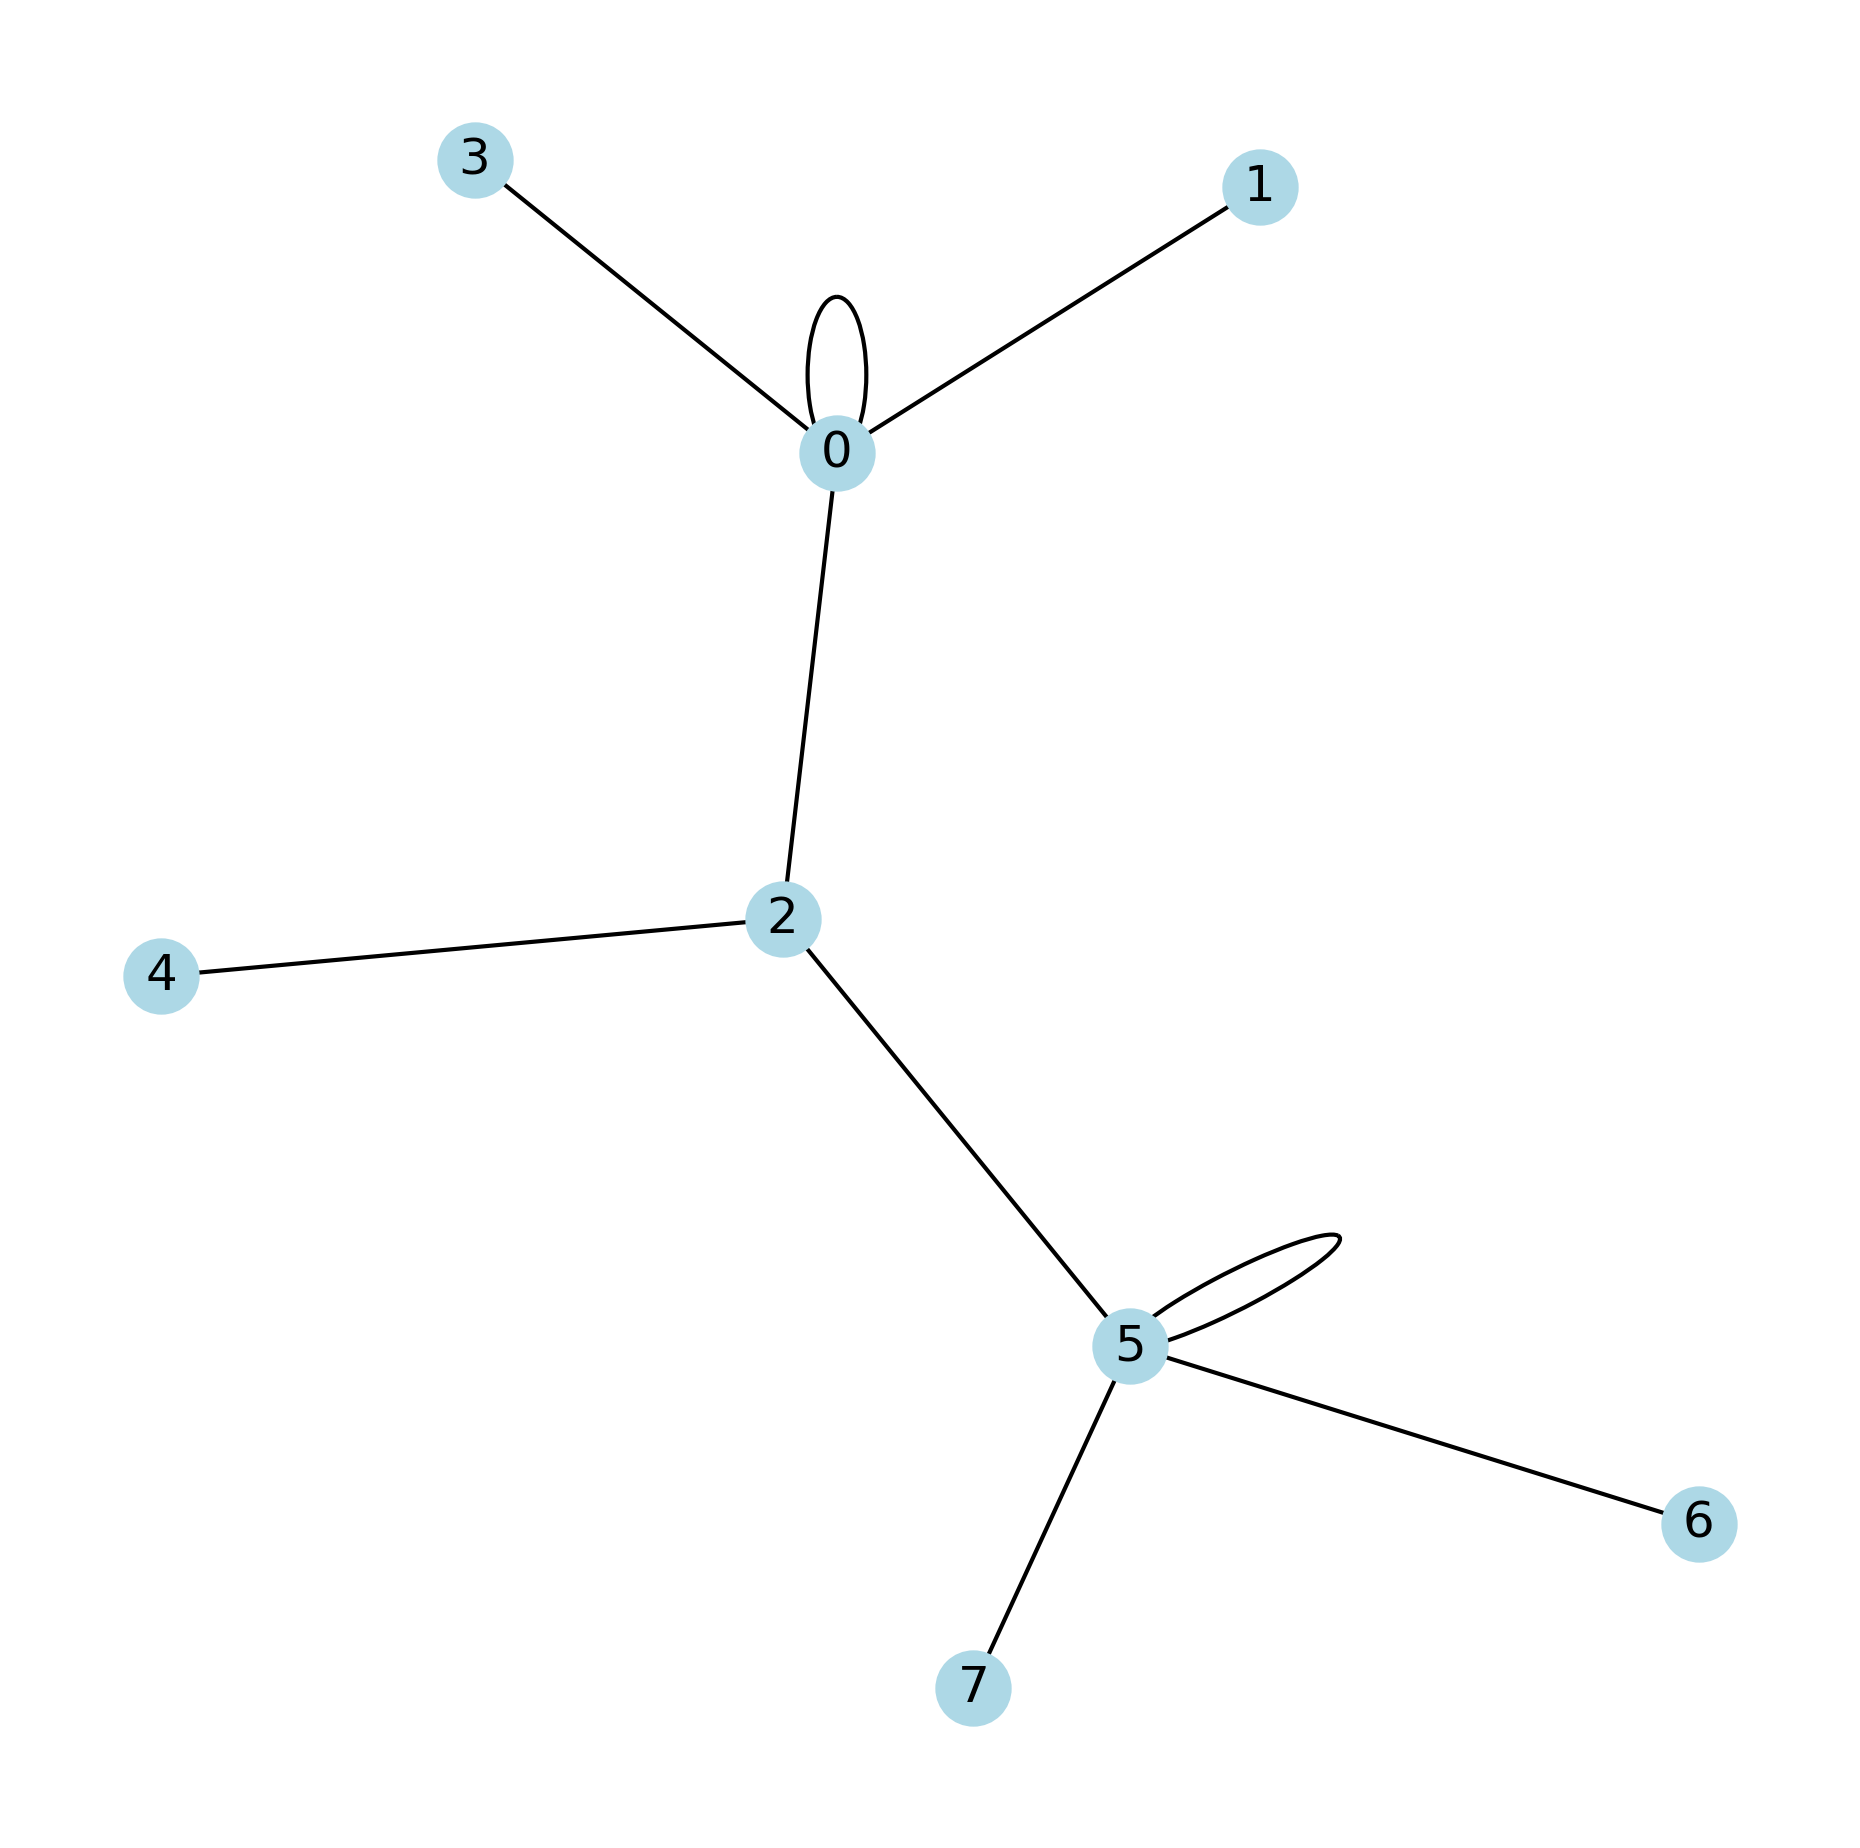
\includegraphics[scale=0.5]{figures/g-004.png}
    \caption{It will become a tree if the loops are removed.}
    \label{fig:4}
\end{figure}

\begin{theorem} \label{thm:3}
    If graph $T$ is loopless and 
	there exists one and only one path 
	connecting each pair of distinct vertices,
	then $T$ is a tree.
\end{theorem}

\begin{proof}
    First, note that $T$ is connected.
	Assume, on the contrary, 
	there exists a cycle $C$ in  $G$.
	Let  $e$ be an edge in  $C$.
	Since  $T$ is assumed loopless, 
	the two ends of  $e$ must be distinct, say  $x$ and $y$.

	Note that there exists a $(x,y)$-path in  $C - e$,
	which is different from the path $xy$. 
	(In fact, this path is $C-e$ itself.) 
	This leads to a contradiction.
\end{proof}

%------------------------------

\begin{theorem} \label{thm:4}
    Let $T$ be a tree. Then we have 
	\begin{align}
		\abs{E} = \abs{V} - 1
		\label{eq:10}
	\end{align}
\end{theorem}

\begin{proof}
	We shall prove by induction on the order $\abs{V}$.

	\noindent\textbf{Base Case:} If $\abs{V} = 1$, 
	then $T$ is a trivial graph without any edges, 
	and hence \eqref{eq:10} holds.

	\noindent\textbf{Inductive Step:} Assume this theorem 
	holds for any trees with order $k$.
	Suppose now $\abs{V(T)} = k+1$.
	Pick a vertex $v$ with $\deg(v) = 1$, and then remove it from $T$.
	This is always possible as we have noted.
	Observe that  $T - v$ remains a tree.
	And by removing $v$, 
	we only remove a single edge from  $T$ since  $\deg(v) = 1$.
	Therefore, $\abs{E(T-v)} = \abs{E(T)} - 1$.
	But by the induction hypothesis, 
	we know $\abs{E(T-v)} = \abs{V(T-v)} - 1 = k - 1$. 
	It then follows that 
	 \begin{align*}
		 \abs{E(T)} = \abs{E(T-v)} + 1 
		 = k-1+1
		 = (k+1)-1 
		 = \abs{V(T)} - 1
	\end{align*}
	This completes the proof.
\end{proof}

%==============================

% references
\printbibliography[heading=bibintoc, title=References]

%==============================

% print index page
\printindex

%==============================

\end{document}
